\documentclass[10pt]{article}

\usepackage{amsmath}% http://ctan.org/pkg/amsmath
\usepackage{amsthm}
\usepackage{todonotes}
\usepackage[margin=1in]{geometry}
\usepackage{algorithm}
\usepackage{url}
\usepackage[noend]{algpseudocode}
\usepackage{mdframed}
\usepackage{tikz}
\usepackage{enumerate}
\usetikzlibrary{matrix,shapes,arrows,positioning,chains, calc}

%% defining new theorem environment for definition
\newtheorem{defn}{\textbf{Definition}}
\newtheorem{thm}{\textbf{Theorem}}
\newtheorem{cor}{\textbf{Corollary}}
\newtheorem{lemma}{\textbf{Lemma}}

\renewcommand{\algorithmicrequire}{\textbf{Input:}}
\renewcommand{\algorithmicensure}{\textbf{Output:}}

\begin{document}
\title{IP-to-NDN Gateway Application-Layer Middleware}
\author{Christopher A. Wood \\ {\tt woodc1@uci.edu}}
\date{\today}
%\thanks{TODO}
\maketitle

%%%%%%%%%%%%%%%%%%%%%
%%% MAIN CONTENT
%%%%%%%%%%%%%%%%%%%%%

\section{Introduction}
Today's Internet architecture is largely inspired by traditional communication-based switching networks. Consequently, it has been retrofitted with a variety of transport and application layer protocols and middleware to support a growing set of consumer applications. Of particular importance are content distribution applications, such as media streaming services similar (e.g., Netflix), which leverage the underlying communication-based network as a distribution network and continue to consume vital networking resources at a rapidly increasing pace. Information-centric networks (ICNs) are a new class of network architectures that aim to address this increasingly popular type of network traffic by decoupling data from its source and shifting the emphasis of addressable content from hosts and interfaces to content \cite{}. By directly addressing content instead of hosts, content dissemination and security can be decoupled from the source and distributed throughout the network. 

Currently, several information-centric networking proposals are being explored as alternative designs to today's public Internet, including MobilityFirst \cite{}, XIA \cite{}, Named Data Networking (NDN) \cite{NDNtech}, ChoiceNet \cite{}, and Nebula \cite{}; the development of each is still an area of active research. As a replacement for IP-based networks, the complete adoption of any one of these designs will realistically be done in by slow and continual integration and replacement of IP-based networking resources with ICN-based resources. Currently, however, there is no engineering plan to support the IP-to-NDN integration. 

Consequently, the primary objective of this project is to aid the integration of future content-centric networking resources into the existing IP-centric Internet by providing an application-layer gateway between IP and NDN resources. Application-layer traffic corresponding to protocols such as HTTP, FTP, SMTP, IMAP, etc. will be translated by middleware running in such gateways to correctly interface with the NDN resources. 

\section{Overview}
TODO: figure and expansion

% \begin{figure}
% \begin{center}
% 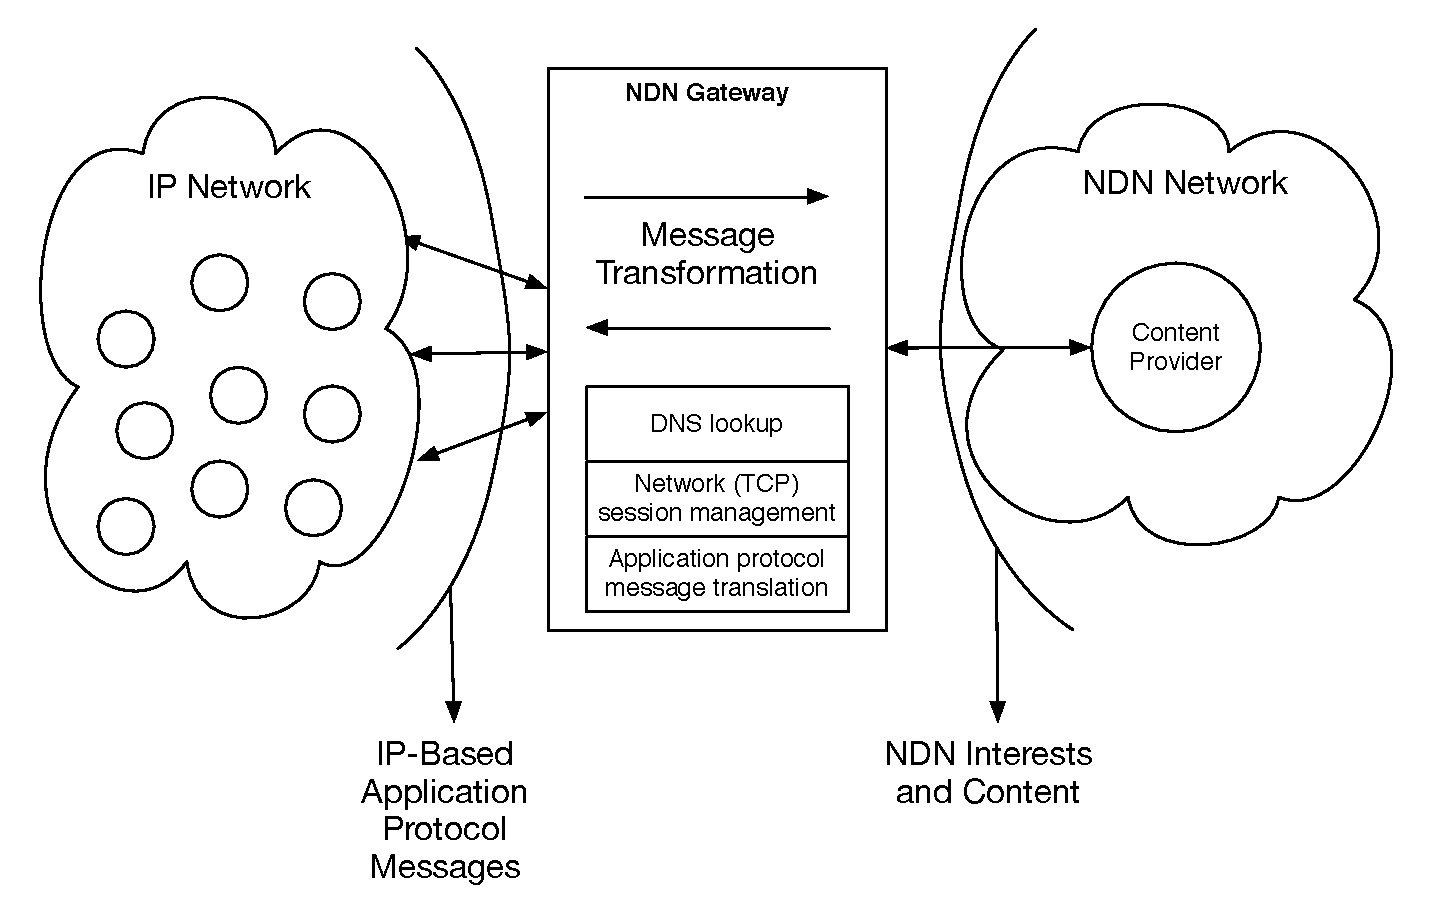
\includegraphics[scale=0.5]{images/gateway_highlevel.pdf}
% \end{center}
% \end{figure}

\section{Implementation}
TODO: java IP-based front-end running listeners for all supported application-layer protocols, C-based backend using NDNx (CCNx), local DNS lookup and translation for each protocol

\section{Deliverables and Time-Line}
TODO

{\bf Deliverables:}
\begin{itemize}
	\item Application gateway source code
	\item Web interface (for gateway configuration)
\end{itemize}

{\bf Timeline:}
\begin{enumerate}[{\bf Week} 1:]
	\setcounter{enumi}{2}
	\item Project proposal and preliminary project experiments
	\item Front-end skeleton, API design, and application-layer protocol listeners
	\item Back-end skeleton, design, and NDNx integration
	\item Java JNI integration and application-wide integration testing
	\item Middleware DNS lookup
	\item Middleware session management
	\item Middleware application layer translation
	\item Elementary web interface and finalize project experiments
	\item Conduct experiments and draft final report 
\end{enumerate}

%%%%%%%%%%%%%%%%%%%%%
%%% END MAIN CONTENT
%%%%%%%%%%%%%%%%%%%%%

%%% BIBLIOGRAPHY
\begin{thebibliography}{[MT1]}

\bibitem{NDNtech} TODO

\end{thebibliography}

\end{document}
